\chapter{Daten und Messungen}
\label{chap:dataandmeasure}

%%%%%%%%%%%%%%%%%%%%%%%%%%%%%%%%%%%%%%%%%%%%%%%%%%%%%%%%%%%%
\section{Mobile iBeacons}
\label{sec:dataandmeasurement:mobilebeacon}
%%%%%%%%%%%%%%%%%%%%%%%%%%%%%%%%%%%%%%%%%%%%%%%%%%%%%%%%%%%%
Die mobilen iBeacon verzichten, wie der Name schon andeutet, auf eine feste Stromquelle und werden ausschließlich mit Batterien betrieben.
Zum Einsatz kommen dabei die sogenannten Knopfzellen, welche mit einer Spannung von 3,0 Volt operieren.
Da Bluetooth Low Energy extrem energiesparend arbeitet, geben die Hersteller der Beacons, die Akkulaufzeit mit bis zu zwei Jahren, ohne einen Batteriewechsel, an. Diese Laufzeit hängt jedoch mit der gewählten Signalstärke und dem Sendeintervall zusammen, welche diese sehr stark beeinflussen können.

Bisher gibt es nur wenige Hersteller von iBeacons, wobei sich der Großteil der Produkte momentan noch in der Entwicklungsphase befindet. Die genutzten iBeacons von \emph{estimote} und \emph{kontakt.io} sind ebenfalls noch in der Entwicklungsphase und wurden hauptsächlich als Testgeräte für Entwickler ausgegeben. Dabei bleibt unklar inwieweit sich das fertige Produkt in den technischen Spezifikationen und der Leistung von den aktuellen Prototypen unterscheiden wird.

%%%%%%%%%%%%%%%%%%%%%%%%%%%%%%%%%%%%%%%%%%%%%%%%%%%%%%%%%%%%
\subsection{estimote Beacon}
\label{sec:dataandmeasurement:mobilebeacon:estimote}
%%%%%%%%%%%%%%%%%%%%%%%%%%%%%%%%%%%%%%%%%%%%%%%%%%%%%%%%%%%%
Die Firma \emph{estimote} \cite{estimote} mit Sitz in Polen, war eine der ersten, welche ein funktionstüchtiges iBeacon vorgestellt hat und es in einem \emph{Developer Preview Kit} zum Verkauf anbieten.
Dieses Kit beinhaltet drei verschiedenfarbige Beacons, welche mit einer wiederverwendbaren Klebeschicht an der Unterseite ausgestattet sind. Dies erlaubt ein beliebiges Anbringen und Abziehen der Beacons auf allen glatten Oberflächen.
\begin{figure}[htb!]
		\centering
	\includegraphics[scale=0.1]{estimote-developer-kit}
	\caption{Das Developer-Kit von estimote}
	\label{estimote-developer-kit}
\end{figure}

Im Inneren des Beacons befindet sich der nRF51822 Bluetooth-Chipsatz von Nordic Semiconductor \cite{nordicchipset}, welcher auf einem 32-bit ARM Prozessor beruht und mit einem 2,4Ghz Bluetooth Low Energy Modul arbeitet. Dabei verfügt der über 256 KB Flash-Speicher für Speicherung der Beacon-Konfiguration \cite{estimotespecs} .
In den estimote Beacons wurde zusätzlich noch ein Temperatursensor und ein Accelerometer integriert, welche sich jedoch softwareseitig noch nicht ansprechen lassen.

Des Weiteren stellt estimote noch ein SDK für Android und iOS zur Verfügung, welches in Fall des iOS-SDK auf der iBeacons-API basiert, jedoch speziell auf die estimote-Beacons abgestimmt ist \cite{estimoteapi} . 
Dabei bietet es neben den Funktionen der iBeacon-API noch die Funktionalität, sich mit den estimote Beacons zu verbinden und deren Konfiguration anzupassen. So erlaubt es zum Beispiel die Signalstärke, das Sendeintervall und die Major-Minor-Informationen zu verändern oder die Firmware der Beacons zu aktualisieren.

Da das SDK, bis auf die Programmierung der Beacons, keine Vorteile gegenüber dem Core Location-Framework mit der iBeacons-API bietet, wurde jedoch auf die Verwendung verzichtet.

%%%%%%%%%%%%%%%%%%%%%%%%%%%%%%%%%%%%%%%%%%%%%%%%%%%%%%%%%%%%
\subsection{kontakt.io Beacon}
\label{sec:dataandmeasurement:mobilebeacon:kontaktio}
%%%%%%%%%%%%%%%%%%%%%%%%%%%%%%%%%%%%%%%%%%%%%%%%%%%%%%%%%%%%
Ein weiteres Unternehmen, welches sich eine eigene iBeacons-Lösung anbietet ist \emph{kontakt.io}. Auch hier ist noch kein finales Produkt erhältlich, sondern nur ein \emph{Development Kit}, welches zehn Beacons enthält. 
Die Beacons sind relativ schlicht gehalten und das Innere ist sehr einfach zugänglich, sodass ein Batteriewechsel ohne Umstände möglich ist.


\begin{figure}[htb!]
		\centering
	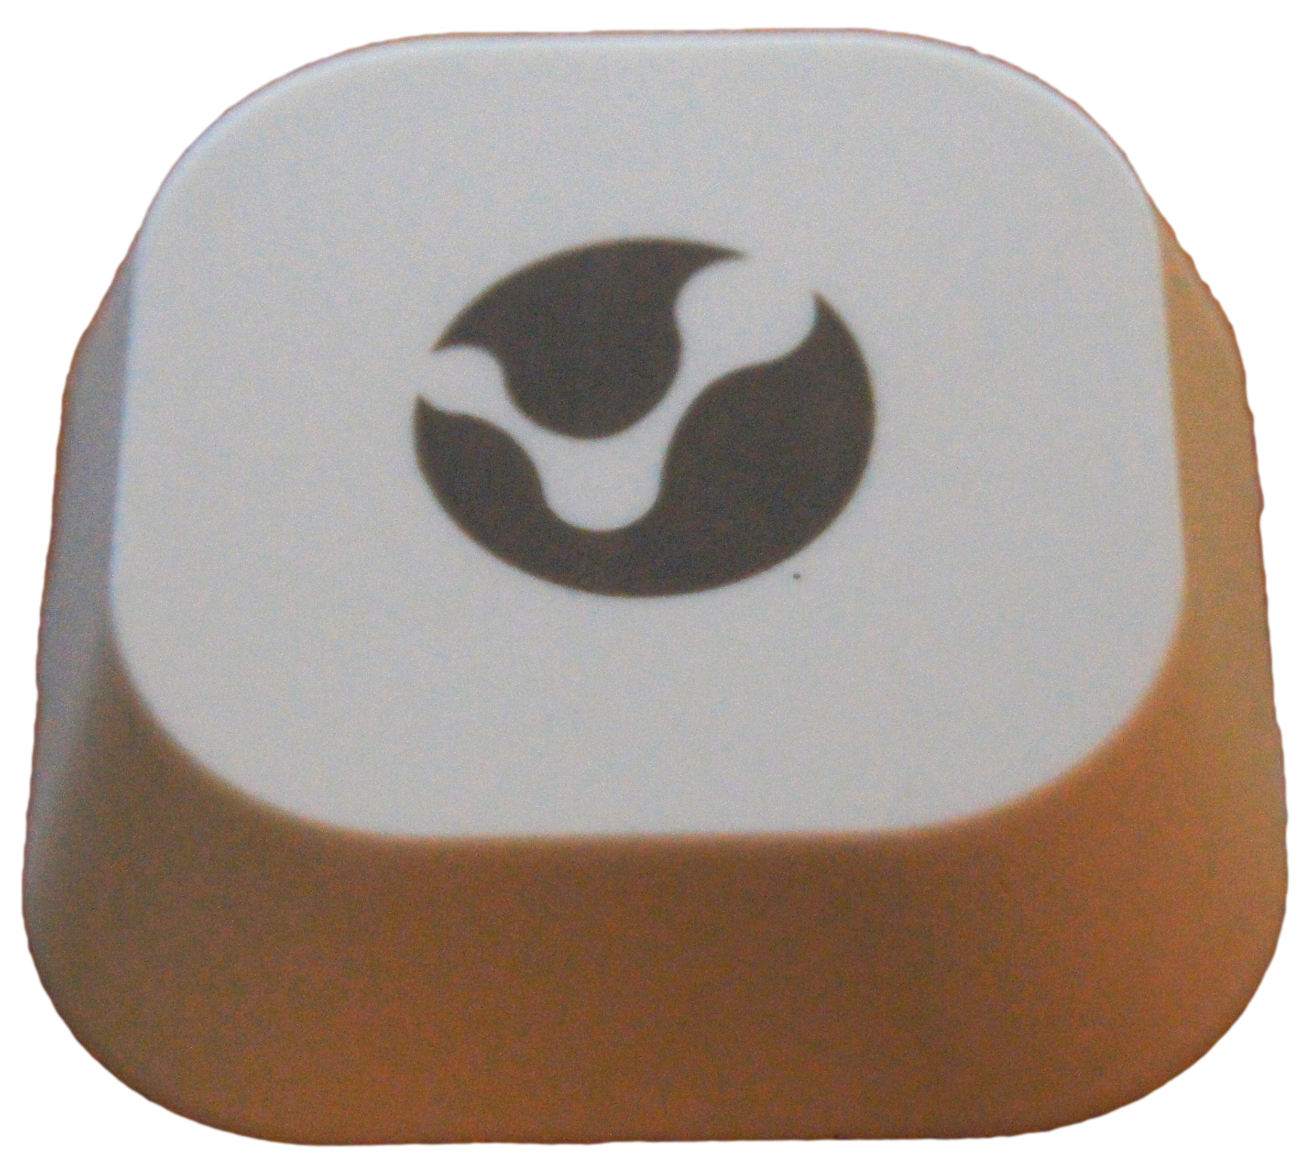
\includegraphics[scale=0.1]{kontakt-beacon-outside}
	\caption{Kontakt.io Beacon}
	\label{kontakt-beacon-outside}
\end{figure}

Die Beacons von \emph{kontakt.io} basieren dabei auf dem BLE113 Chipsatz von \emph{bluegiga} \cite{bluegigachipset}. Die Beacons verfügen dabei einen ARM Cortex M0 Porzessor mit 256 KB Flashspeicher. Die Ausgangssignalstärke des Chipsatz lässt sich zwischen +4dBm und -20dBm variabel einstellen.


Auch kontakt.io bietet eine eigene API an, welches im Gegensatz zu dem SDK von \emph{estimote} nicht nativ für die einzelnen Plattformen entworfen wurde, sondern online über eine REST-Schnittstelle arbeitet \cite{kontaktapi}.
Dabei stellt \emph{kontakt.io} ein Webpanel zur Verfügung, in welchem man die einzelnen Beacons mit ihrem UUID, Major und Minor-Wert registriert und jedem den jeweiligen Ort beziehungsweise eine Funktion zuweisen kann. 
Auch auf die Verwendung dieses SDK wurde verzichtet, da es nicht dem geplanten Anwendugszweck gerecht wird.


%%%%%%%%%%%%%%%%%%%%%%%%%%%%%%%%%%%%%%%%%%%%%%%%%%%%%%%%%%%%
\section{Stationäre iBeacons}
\label{sec:dataandmeasurement:stationarybeacon}
%%%%%%%%%%%%%%%%%%%%%%%%%%%%%%%%%%%%%%%%%%%%%%%%%%%%%%%%%%%%
Neben den mobilen iBeacons, welche mittels Batterien betrieben werden, gibt es auch stationäre iBeacons, welche auf eine stetige Anbindung an das Stromnetz angewiesen sind.
Dabei gibt es verschiedene Ansätze.
Zum Einen bieten zum Beispiel \emph{PayPal} und \emph{Radius Networks} einen Ansatz, bei dem die komplette Technik in einen USB-Stick integriert wird und über ein USB-Netzteil an jeder Steckdose betrieben werden kann. Diese Beacons basieren dabei auf den gleichen Chipsätzen wie auch ihre batteriebetriebenen Pendants.

Eine andere Lösung ist die Nutzung eines Bluetooth 4.0-kompatiblen USB-Dongles an einem Computer. Dieser kann mit entsprechender Software zu einem iBeacon umfunktioniert werden.

%%%%%%%%%%%%%%%%%%%%%%%%%%%%%%%%%%%%%%%%%%%%%%%%%%%%%%%%%%%%
\subsection{Raspberry Pi als iBeacon}
\label{sec:dataandmeasurement:stationarybeacon:raspberrypi}
%%%%%%%%%%%%%%%%%%%%%%%%%%%%%%%%%%%%%%%%%%%%%%%%%%%%%%%%%%%%
Der Raspberry Pi ist ein Mini-Computer, welcher auf dem BCM2835 ARM-Prozessor von Broadcom basiert und als günstiger Computer für Programmiereinsteiger konzipiert wurde \cite{raspberrypi}. Der kleine Computer ermöglicht aber auch andere Einsatzgebiete, zum Beispiel als Beacon.

Um den Raspberry Pi zu einem Beacon umzufunktionieren wurde eine Linux-Distribution auf dem Gerät installiert und ein Bluetooth-Dongle über USB angeschlossen. Dabei kam das USB-BT4LE Bluetooth 4.0-Modul von \emph{Plugable Technologies} zum Einsatz, welches spezielle Bluetooth 4.0 und Linux-Unterstützung bietet \cite{plugable}.
Für die Umfunktionierung zum iBeacon wurde die Bluetooth-Implementierung \emph{blueZ} eingesetzt, welche es erlaubt das Bluetooth-Modul anzusprechen und spezifische Nachrichten über Bluetooth zu versenden \cite{bluez}.
Diese Möglichkeit den Raspberry Pi als iBeacon zu nutzen, wurde von der Firma Radius Network vorgestellt. Diese bieten ein ausführliches Tutorial für die Nutzung des Raspberry Pi als iBeacon auf ihrer Webseite an \cite{radiusraspberry}, welches von mir genutzt wurde, um den Raspberry Pi zu konfigurieren.

Radius Network hat dabei den Nachrichteninhalt der iBeacons-Mitteilungen mittels Reverse-Engineering aufgeschlüsselt. Dies ermöglicht eine Reproduzierung der Nachricht mit eigenen Parametern für die UUID, Major und Minor-Werte.

%%%%%%%%%%%%%%%%%%%%%%%%%%%%%%%%%%%%%%%%%%%%%%%%%%%%%%%%%%%%
\section{Physikalische Grundlagen}
\label{sec:dataandmeasurement:physics}
%%%%%%%%%%%%%%%%%%%%%%%%%%%%%%%%%%%%%%%%%%%%%%%%%%%%%%%%%%%%
Im Vergleich zu Kabelverbindungen, wo die Ausbreitung des Signals entlang eines bestimmten Leiters geschieht, ist die Ausbreitung eines drahtlosen Signals von deutlich mehr Faktoren abhängig \cite{signalverbreitung}. 

\textbf{Dämpfung}

Dämpfung ist die Schwächung der Energie, mit welcher das Signal übertragen wird. Diese tritt auch bei einer freien Sichtverbindung zwischen Sender und Empfänger auf. Die Verringerung der Leistung ist dabei abhängig von der Ausgangssendeleistung $P_0$ und der Entfernung $r$ zwischen Sender und Empfänger. Die letztlich am Empfänger ankommende Signalstärke $P_r$ berechnet sich dabei wie folgt:

\begin{equation}
	P_r = \frac{P_0}{r^{2}} 
\end{equation}

Die Abschwächung des Signals resultiert aus der Art der Aussendung. Da die hier verwendeten Beacons einem Punktstrahler entsprechen, wird die anliegende Signalstärke auf eine Kugeloberfläche verteilt. Die Kugeloberfläche $O$ lässt sich dabei abhängig vom Radius $r$ mittels der Formel $O = 4 \pi r^{2}$ berechnen. Die Oberfläche vergrößert sich damit quadratisch zum Radius.

\textbf{Abschattung}

Die Abschattung ist eine stärkere Form der Dämpfung, welche durch Objekte zwischen der Signalquelle und dem Empfänger verursacht wird. Die Abschattung ist dabei abhängig von der Frequenz des Signals und der Geschaffenheit des Objektes. Eine höhere Frequenz des Signals führt dabei zu einer stärkeren Abschattung.

\textbf{Reflexion}

An größeren Oberflächen kann es zu Reflexionen des Signals kommen. Dabei trifft es auf die Oberfläche und wird dann in abgeschwächter Form reflektiert.

\textbf{Streuung}

Die Streuung ähnelt der Reflexion, da auch hier das Signal reflektiert wird. Während dieses Vorganges wird das Signal jedoch aufgespalten und dadurch in verschiedene Richtungen abgelenkt.

\textbf{Mehrwegeausbreitung}

Durch die oben genannten Effekte ist es möglich, dass ein Signal einen Empfänger auf mehreren Wegen erreicht. Dabei ist die Signalstärke stark abhängig von dem zurückgelegtem Weg. Ausserdem unterscheiden sich die Laufzeiten der Signale, da diese ebenfalls vom Weg abhängig sind. Dadurch kann es auch zu Überlagerungen zwischen Signalen kommen, welche zur gleichen Zeit gesendet wurden, jedoch zu unterschiedlichen Zeiten beim Empfänger eintreffen. 
Durch diese Phasenverschiebung kann das Signal zusätzlich abgeschwächt werden.


%%%%%%%%%%%%%%%%%%%%%%%%%%%%%%%%%%%%%%%%%%%%%%%%%%%%%%%%%%%%
\section{Innenraummessungen}
\label{sec:dataandmeasurement:indoormeasure}
%%%%%%%%%%%%%%%%%%%%%%%%%%%%%%%%%%%%%%%%%%%%%%%%%%%%%%%%%%%%
Um die Leistungsfähigkeit und das Verhalten der Beacons in Innenräume zu testen und darzustellen, wurden verschiedene Messungen durchgeführt. Dazu wurden zum einen die mobilen Beacons verwendet und zum Anderen der Raspberry Pi, als stationäres Beacon.
Die Messungen wurden dabei sowohl mit dem iPhone 5 als auch mit dem iPhone 4s durchführt, um auch hier die Unterschiede zwischen den einzelnen Modellen zu erfassen.


Zuerst wurden die Messungen mit den mobilen Beacons, hier die \emph{kontakt.io}-Beacons, durchgeführt.
Diese wurden in einem leeren Raum durchgeführt, wobei immer freie Sicht zwischen den Beacons und den Empfangsgeräten bestand. Für jede Entfernung wurden 100 Stichproben genommen, jeweils eine pro Sekunde.
%%%%%%%%%%%%%%%%%%%%%%%%%%%%%%%%%%%%%%%%%%%%%%%%%%%%%%%%%%%%
% figure of signal strnegth
%%%%%%%%%%%%%%%%%%%%%%%%%%%%%%%%%%%%%%%%%%%%%%%%%%%%%%%%%%%%
\begin{figure}[h!]
	\centering
	\begin{minipage}[t]{8cm}
		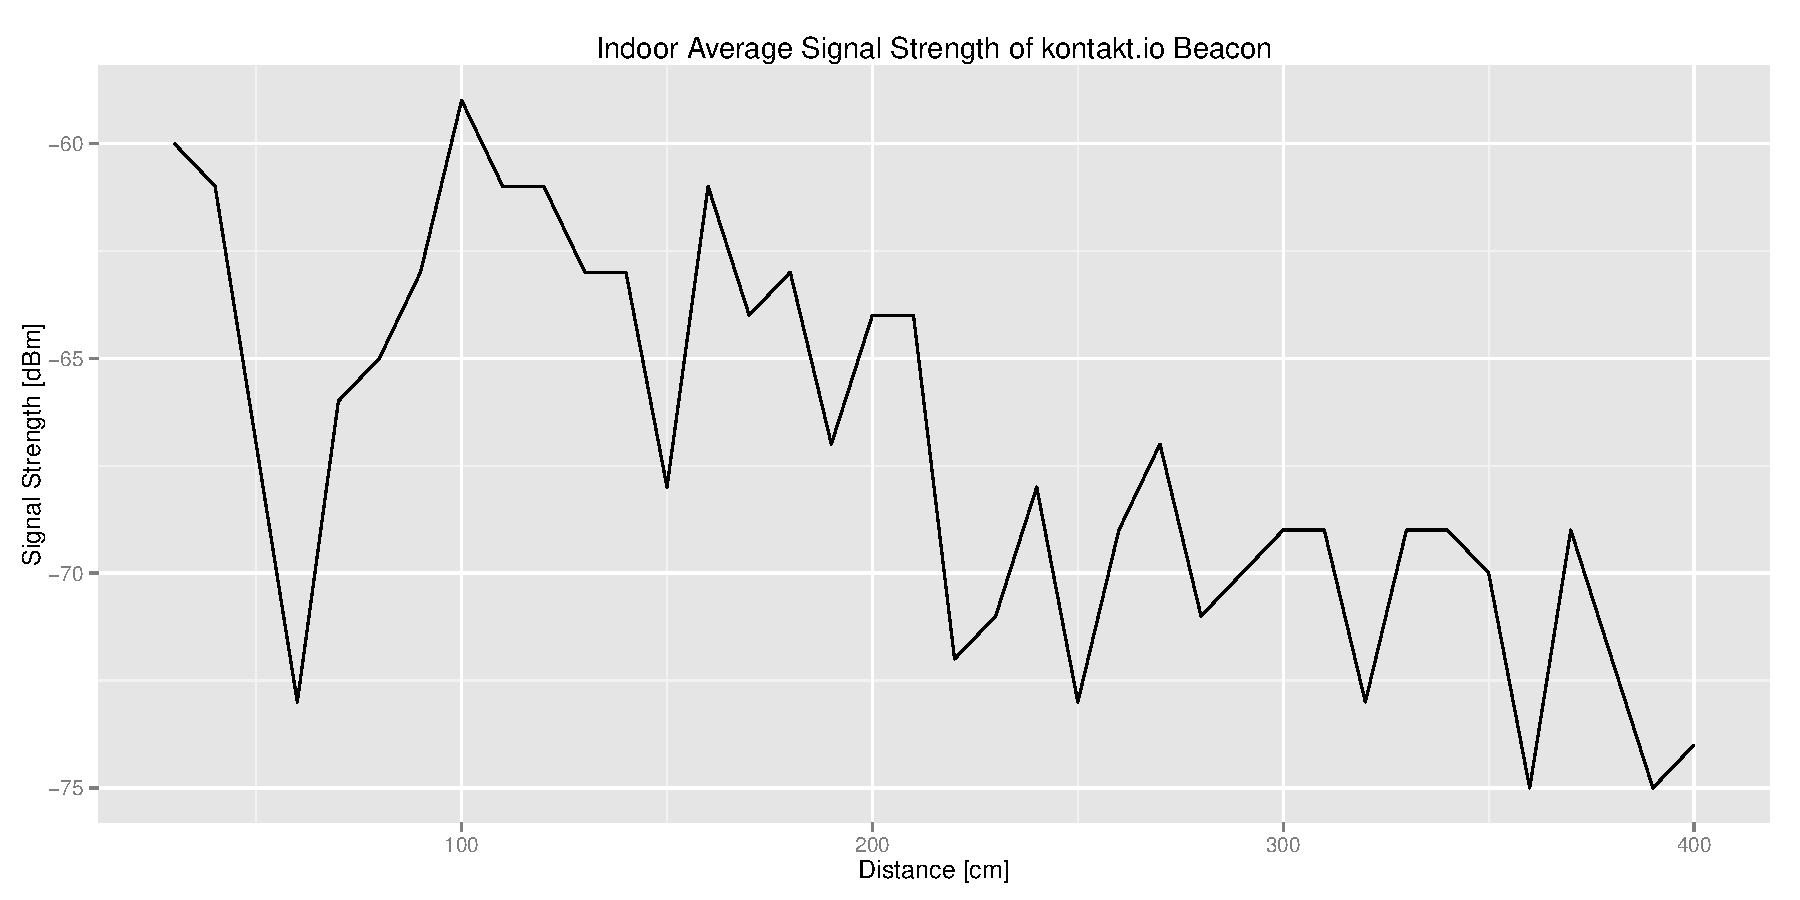
\includegraphics[scale=0.3]{avgiphone5}
		\caption{Messung des iPhone 5}
		\label{avgiphone5-signalstrength}
	\end{minipage}
	\hspace{2cm}
	\begin{minipage}[t]{8cm}
			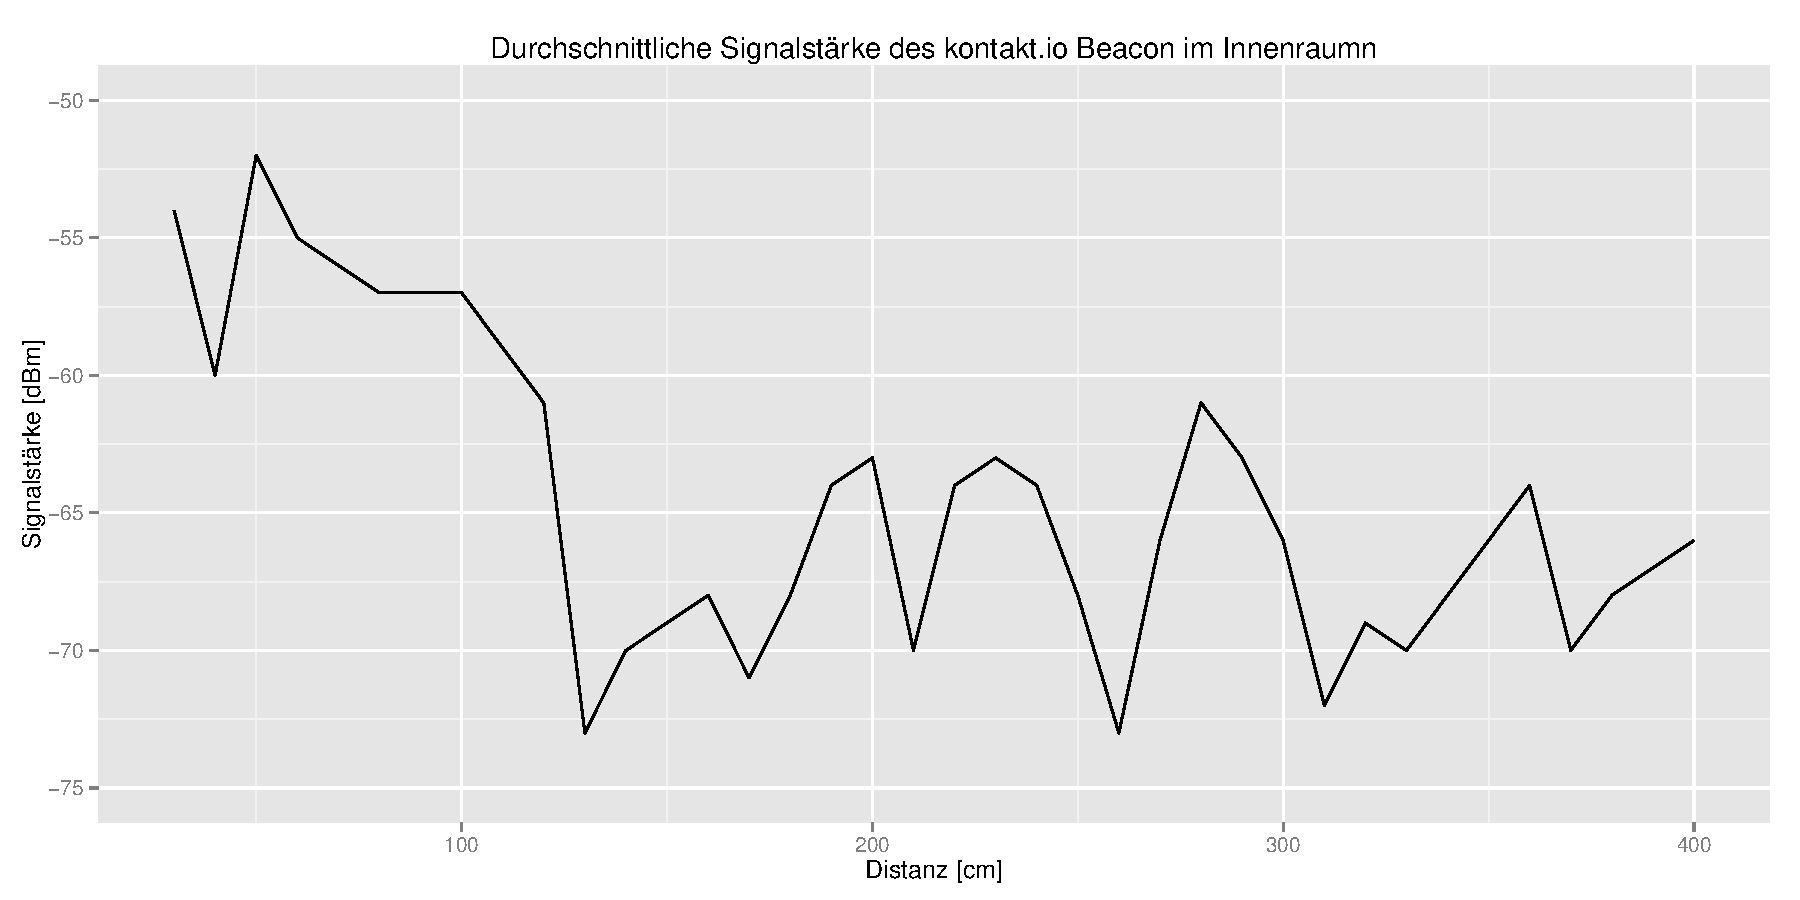
\includegraphics[scale=0.3]{avgiphone4s}
			\caption{Messung des iPhone 4s}
			\label{avgiphone4s-signalstrength}
	\end{minipage}
		\caption{Durchschnittliche Signalstärke eines kontakt.io Beacons}
		\label{signalstrength}
\end{figure}

In Abbildung \ref{avgiphone5-signalstrength} und Abbildung \ref{avgiphone4s-signalstrength} lässt sich dabei sehr gut erkennen, das die Signalstärke, nicht wie eigentlich erwartet stetig abnimmt, sondern relativ stark schwankt. Dies ist darauf zurückzuführen, dass in Innenräumen sowohl Wände, als auch Gegenstände im Raum, das Bluetooth-Signal reflektieren oder blockieren und so die Ergebnisse verfälschen.
Des Weiteren ist zu erkennen, dass die Ergebnisse zwischen den verschiedenen iPhone-Modellen deutlich voneinander abweichen. Das lässt darauf schließen, dass der verbaute Chipsatz, beziehungsweise die verbaute Antenne innerhalb der Gerät, die Ergebnisse deutlich beeinflusst und die Werte daher nur schwer übertragbar sind.

Ein weiterer wichtiger Punkt ist die Untersuchung der Stabilität des Signals. Dabei wurden die gleichen Daten wie zuvor verwendet, jedoch um die minimalen und maximalen Werte ergänzt. In Abbildung \ref{all-iphone5} lässt sich dabei gut erkennen, das die Ergebnisse eine ähnliche Tendenz haben, aber sich dennoch über einen sehr großen Bereich der Signalstärke verteilen.

\begin{figure}[htb!]
		\centering
	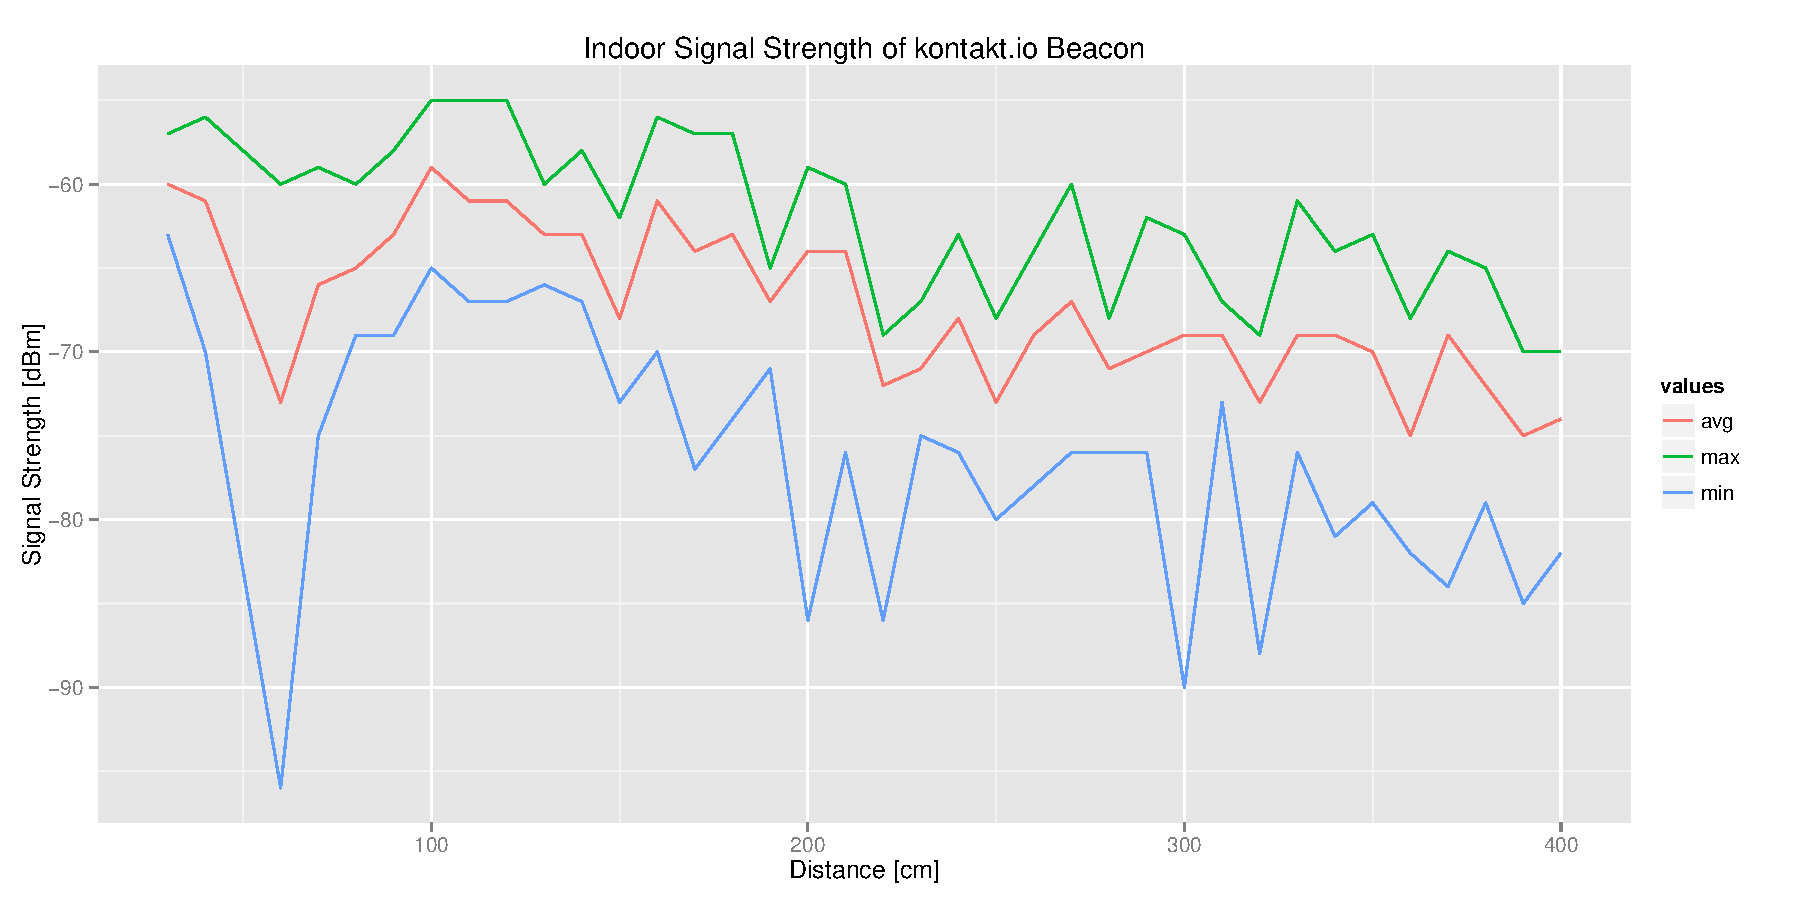
\includegraphics[scale=0.5]{alliphone5}
	\caption{Minimale, maximale und durchschnittliche Signalstärke des Beacons gemessen vom iPhone 5}
	\label{all-iphone5}
\end{figure}


Zusätzlich wurde untersucht, inwieweit sich die Sendeleistung und Signalqualität der batteriebetriebenen Beacon von stationären Beacons unterscheidet.
Dazu wurde der gleiche Messaufbau wie zuvor genutzt, jedoch das \emph{kontakt.io} Beacon durch den Raspberry Pi ausgetauscht. Danach wurden die gleichen Messungen erneut durchgeführt.

\begin{figure}[htb!]
		\centering
	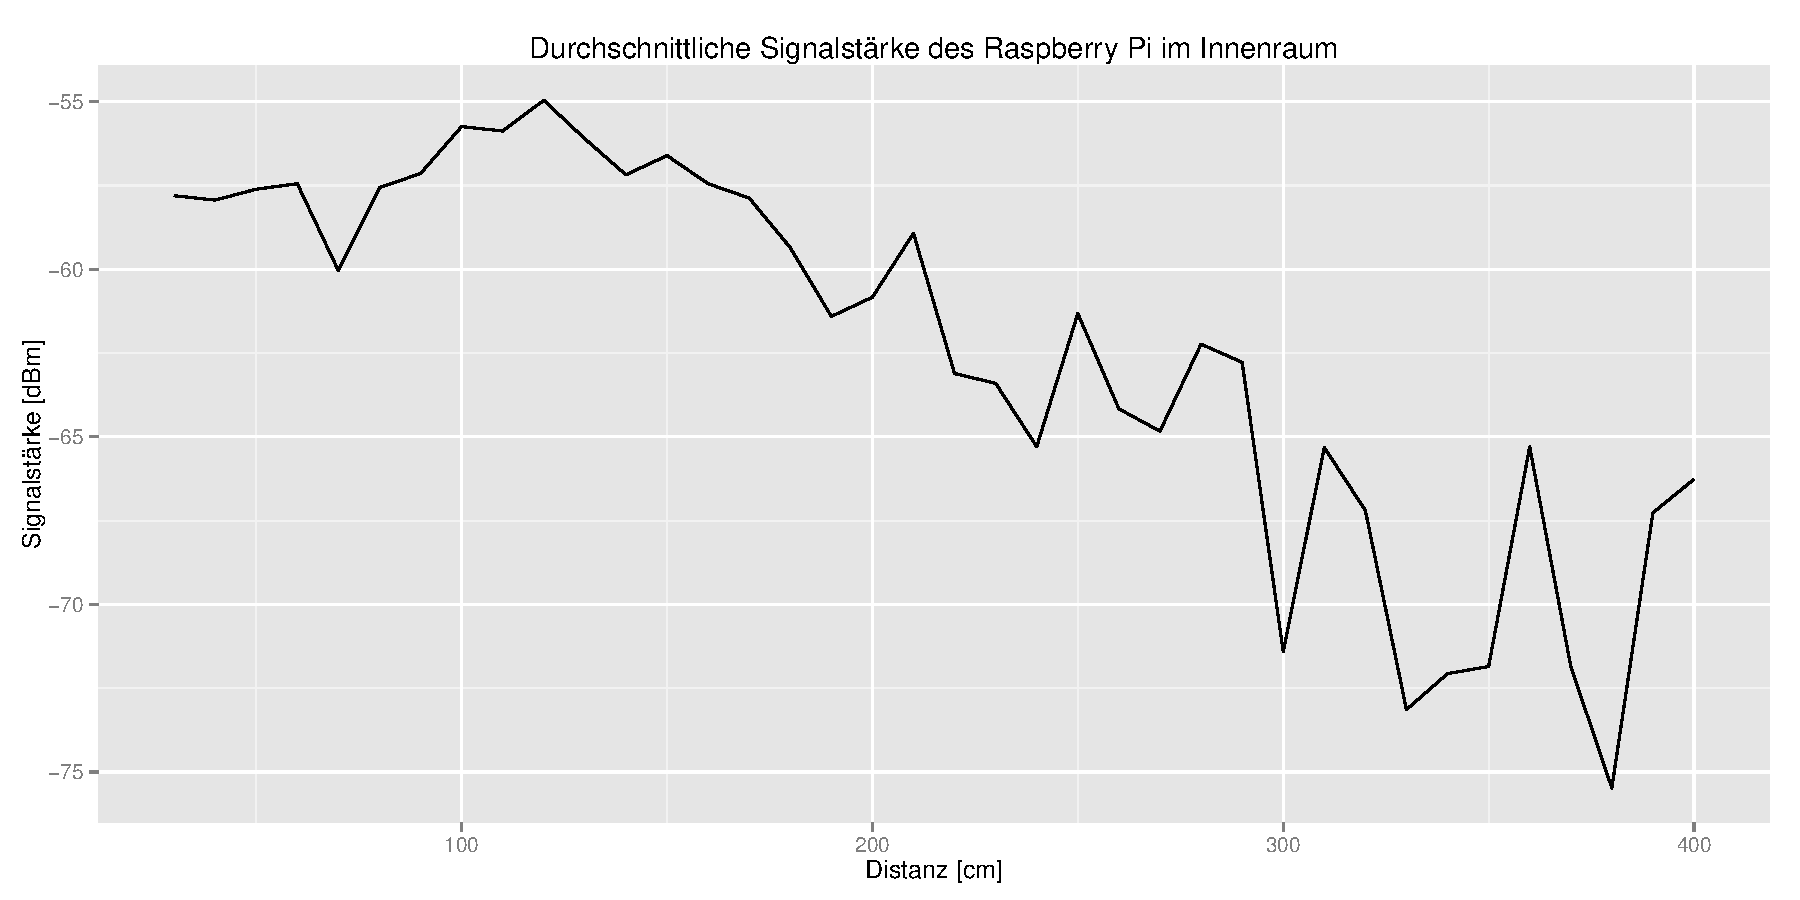
\includegraphics[scale=0.5]{avgiphone5_raspberry}
	\caption{Durchschnittliche Signalstärke des Raspberry Pi Beacons (gemessen mit iPhone 5)}
		\label{avgiphone5_raspberry}
\end{figure}

Wie aus Abbildung \ref{avgiphone5_raspberry} zu entnehmen, sind die Ergebnisse im Vergleich zu der Messung der kontakt.io Beacons näher am erwarteten Ergebnis, welches eine konstante Abnahme der Signalstärke sein sollte. Es sind jedoch immer noch einige Ausreißer zu erkennen. Bei der Betrachtung der minimalen und maximalen Signalstärken fällt auch auf, dass diese ähnlich stark schwanken, wie schon zuvor bei den kontakt.io Beacons. Die Stabilität des Signals des stationären Beacons ist also genauso schwach beziehungsweise noch schwächer, als die des batteriebetriebenen Beacons. Dies wird in Abbildung \ref{alliphone5_raspberry} noch einmal deutlich.

\begin{figure}[htb!]
		\centering
	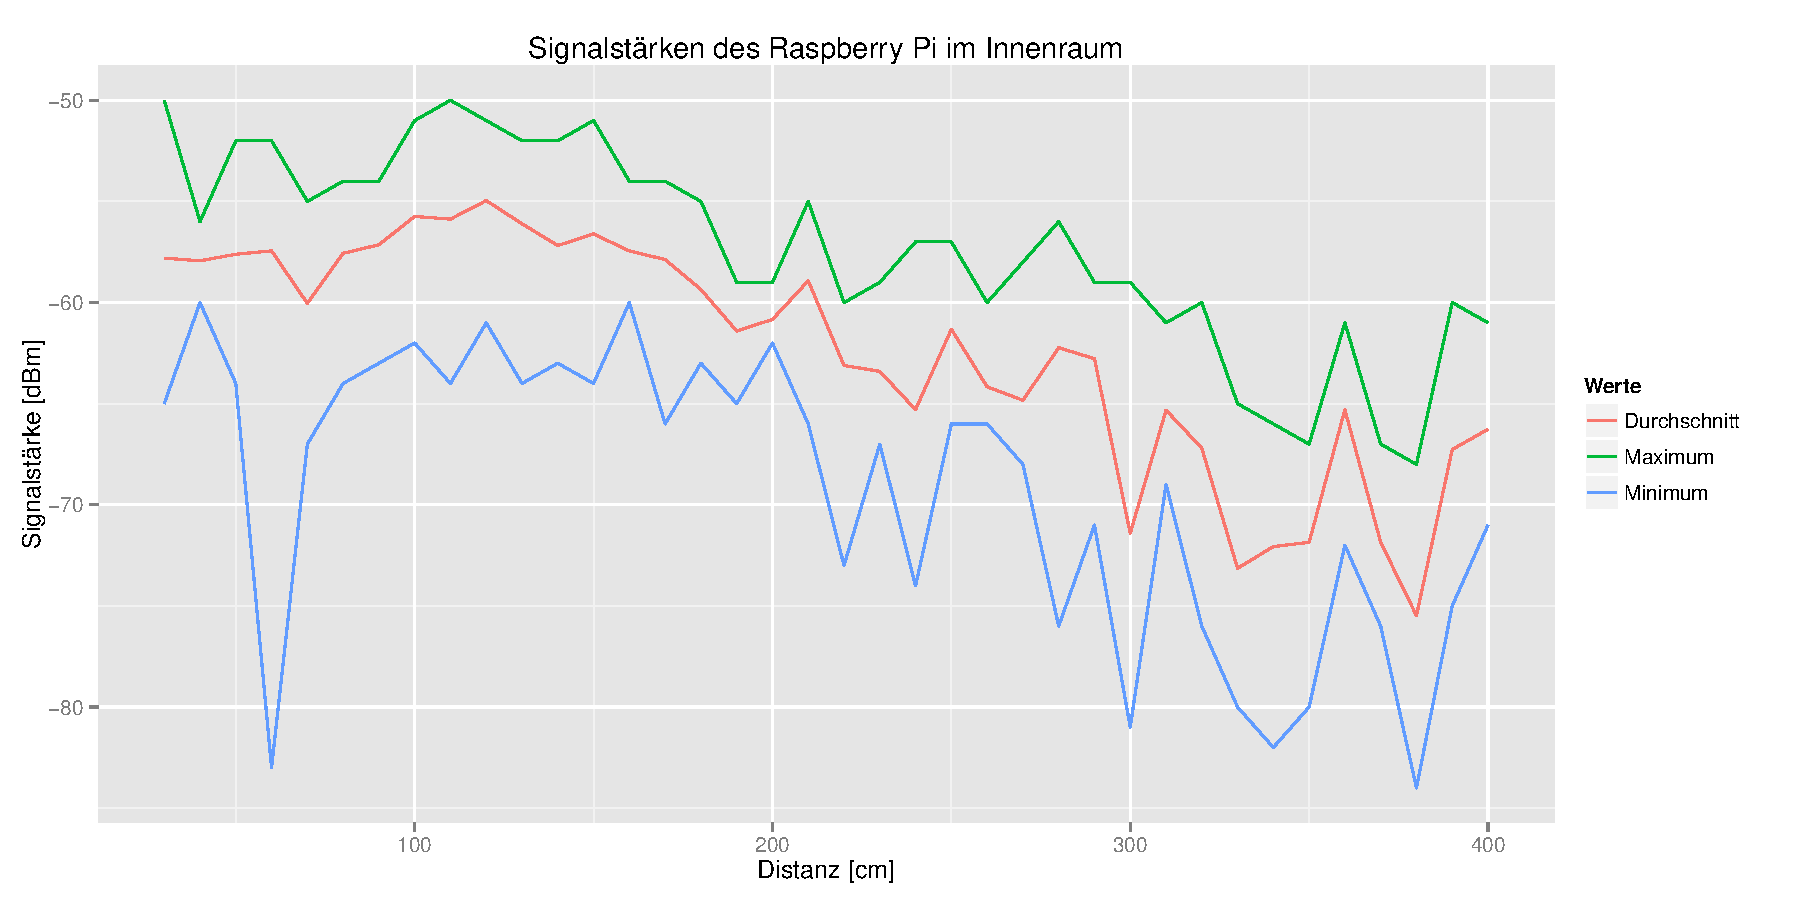
\includegraphics[scale=0.5]{alliphone5_raspberry}
	\caption{Minimale, maximale und durchschnittliche Signalstärke des Raspberry Pi gemessen vom iPhone 5}
	\label{alliphone5_raspberry}
\end{figure}

Für die weiteren Tests und Messungen wurden daher die \emph{kontakt.io} Beacons verwendet, da die beiden zur Verfügung stehenden Beacons sich in Signalstärke und Stabilität nicht zu stark unterscheiden, von den \emph{kontakt.io} Beacons jedoch deutlich mehr Exemplare verfügbar sind und diese variabler im Bezug auf die Positionierung der Beacons sind.


%%%%%%%%%%%%%%%%%%%%%%%%%%%%%%%%%%%%%%%%%%%%%%%%%%%%%%%%%%%%
\section{Mögliche Störfaktoren}
\label{sec:dataandmeasurement:interferencefactor}
%%%%%%%%%%%%%%%%%%%%%%%%%%%%%%%%%%%%%%%%%%%%%%%%%%%%%%%%%%%%
Wie die obigen Messungen zeigen, weichen die realen Ergebnisse stark von den, durch die physikalischen Ausbreitungseigenschaften der elektromagnetischen Wellen, angenommenen Ergebnissen ab. Dies hängt vor allem damit zusammen, dass die Antenne der Beacons nicht gerichtet ist, sondern in alle Richtungen sendet. Dies führt dazu, dass das Signal der Beacons von diversen Flächen im Raum reflektiert und so nicht auf direktem Weg zum Endgerät gelangt. 

Ein weiterer wichtiger Störfaktor ist der Benutzer selbst, da der menschliche Körper größtenteils aus Wasser besteht, welche elektromagnetische Wellen abschirmt. Daher ist zu beobachten, dass die Ausrichtung des Nutzers einen deutlichen Einfluss auf die Signalstärke nimmt. 

\begin{figure}[htb!]
		\centering
	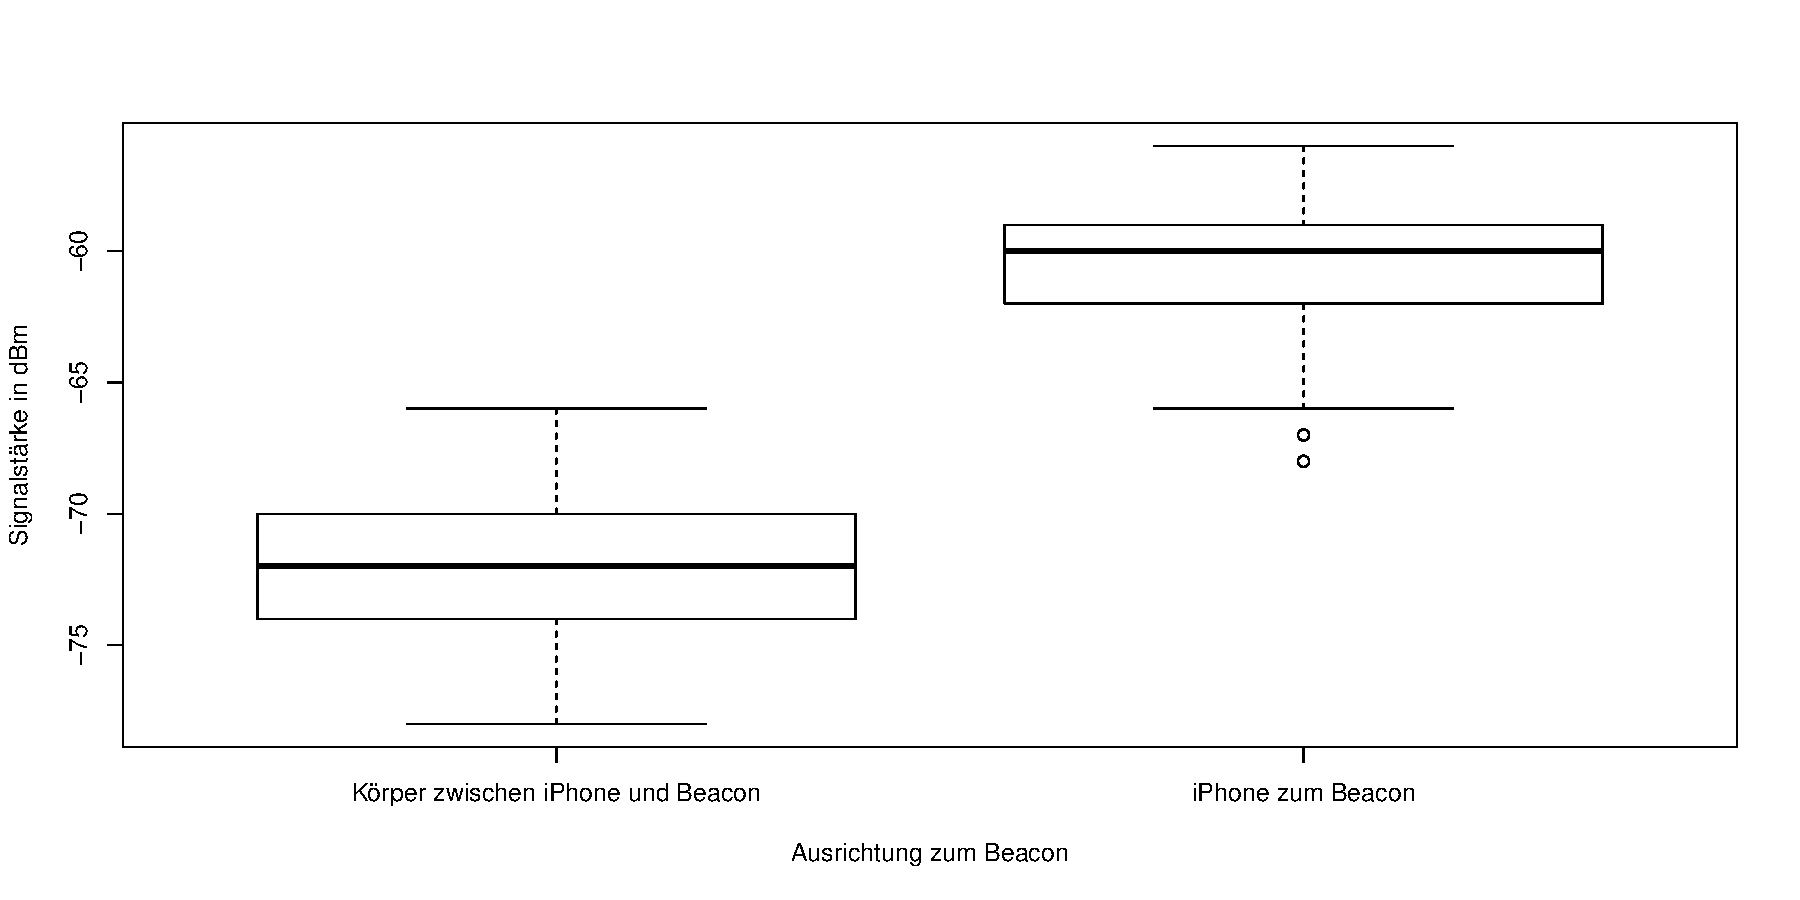
\includegraphics[scale=0.5]{boxplotiPhone5Body}
	\caption{Signalstärke bei 2m Entfernung zum Beacon}
	\label{boxplotiPhone5Body}
\end{figure}

In Abbildung \ref{boxplotiPhone5Body} ist diese Auswirkung des Körpers deutlich zu erkennen. Hierbei wurden jeweils aus zwei Metern Entfernung 100 Stichproben der Signalstärke genommen. Einmal mit freier Sicht zum Beacon und einmal mit dem Körper zwischen Beacon und iPhone. 

Auf der Abbildung ist deutlich zu erkennen, wie der Körper die Signalstärke verringert. Dieser Faktor muss also bei der Positionsbestimmung berücksichtigt werden.

Zusätzlich zum Körper kann es an realen Einsatzorten weitere Gegenstände geben, welche das Signal abschwächen oder komplett abschirmen, wie zum Beispiel Wände oder Möbelstücke.